\documentclass{article}

\usepackage[latin1]{inputenc}
\usepackage{pgfplots}
\usepackage{tikz}
\usetikzlibrary{arrows}

\pgfplotsset{compat=1.10}

\begin{document}
\pagestyle{empty}

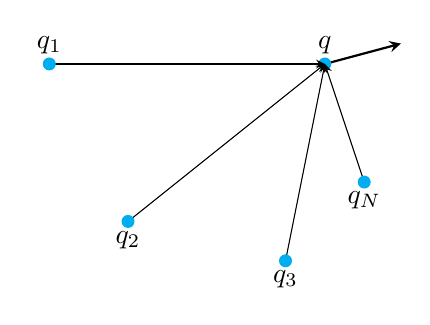
\begin{tikzpicture}[>=stealth]
	\draw[->, thick] (2.5, 2) -- ++(15:1cm);

	\draw[cyan, fill] (2.5, 2) circle [radius=0.075]  node[black, above] {$q$};
	
	\draw[->, thin] (-1, 2) -- (2.5, 2);
	\draw[->, thin] (0, 0) -- (2.5, 2);
	\draw[->, thin] (2, -0.5) -- (2.5, 2);
	\draw[->, thin] (3, 0.5) -- (2.5, 2);

	\draw[cyan, fill] (-1, 2) circle [radius=0.075] node[black, above] {$q_1$};
	\draw[cyan, fill] (0, 0) circle [radius=0.075]  node[black, below] {$q_2$};
	\draw[cyan, fill] (2, -0.5) circle [radius=0.075]  node[black, below] {$q_3$};
	\draw[cyan, fill] (3, 0.5) circle [radius=0.075]  node[black, below] {$q_N$};
\end{tikzpicture}

\end{document}